\jxhj{%教学后记
	}
\skrq{%授课日期
	2017年5月30日 4-5节}
\ktmq{%课题名称
	 自动编程}
\jxmb{%教学目标,每行前面要加 \item
	\item 程序的传输;
	\item 程序的dnc加工;
	\item 自动编程刀路。}
\jxzd{%教学重点,每行前面要加 \item
	\item 程序的传输;
	\item 自动编程刀路。}
\jxnd{%教学难点,每行前面要加 \item
	\item 自动编程刀路。}
\jjff{%教学方法
	通过讲述、举例、演示法来说明;}

\makeshouye %制作教案首页

%%%%教学内容
\subsection{组织教学}
\begin{enumerate}[\hspace{2em}1、]
	\item 集中学生注意力;
	\item 清查学生人数;
	\item 维持课堂纪律;
\end{enumerate}
\subsection{复习导入及主要内容}
\begin{enumerate}[1、]
	\item 简单零件的倒角;
	\item 宏程序实例1;
	\item 宏程序实例2。
\end{enumerate}


\subsection{教学内容及过程}


\subsubsection{数据线的接法}
RS232通讯电缆

RS-232是美国电子工业联盟(EIA)制定的串行数据通信的接口标准,全称是EIA-RS-232(简称232,RS232)。它被广泛用于计算机串行接口外设连接。

RS-232C标准(协议),232是标识号,C代表RS232的最新一次修改(1969年),在这之前,还有RS232B、RS232A

FANUC机床25PIN    电脑 9PIN

Tx(02) ---------->---------- Rx(02)

Rx(03) ----------<---------- Tx(03)

GND(07) ------------------- GND(05)

RTS(04)-CD(08)------>------- CD(01)-CTS(08)

CTS(05) ----------<--------- DTR(04)

DSR(06)<-DTR(20)------>------ DSR(06)

屏蔽 ---------------------- 屏蔽

简化:(不能硬握手)

Tx(02) ----------->--------- Rx(02)

Rx(03) -----------<--------- Tx(03)

GND(07) ------------------- GND(05)

CD(08)-DSR(6)<-DTR(20)         CD(1)DTR(4)->DSR(6)

RTS(4)->CTS(5)                 RTS(7)->CTS(8)

屏蔽 ---------------------- 屏蔽

Siemens 9PIN      电脑9PIN  (只能使用硬握手)

Rx(02)--------<---------Tx(03)

Tx(03)-------->---------Rx(02)

DTR(04)------->---------DSR(06)

GND(05)-----------------GND(05)

DSR(06)-------<---------DTR(04)

RTS(07)-------->--------CTS(08)

CTS(08)--------<---------RTS(07)

Siemens 25PIN      电脑9PIN  (只能使用硬握手)

Rx(02)--------<---------Tx(03)

Tx(03)-------->---------Rx(02)

DTR(06)------->---------DSR(06)

GND(07)-----------------GND(05)

DSR(20)-------<---------DTR(04)

RTS(05)-------->--------CTS(08)

CTS(04)--------<---------RTS(07)

其中:

Tx 发送数据(发)          Rx接受数据(收)

DTR数据终端准备(发)     DSR数据准备好(收)

RTS请求发送          CTS清除发送

CD 数据载波检测

Tx、DTR和RTS信号是由数据终止设备(DTE)产生的,Rx、DSR、CTS、DCD信号是由数据通讯设备(DCE)产生的。

DCE(如打印机)-------DTE(如服务器)

连接两个DTE设备需要一个虚拟调制解调器来充当DCE,需交换相应的信号(TD-RD, DTR-DSR, and RTS-CTS),就是上面的接法。

握手是在通信电路建立之后,信息传输开始之前。 握手用于达成参数,如信息传输率,字母表,奇偶校验, 中断过程,和其他协议特性。

软件握手(XON/XOFF)------握手通过交换的打印机与通过在传输服务器之间的控制代码来实现的并分别接收行。 数据通讯设备的数据缓冲区满时它会发送通知服务器的打印处理器的 XOFF 暂停输出。 当缓冲区可用空间的更多的数据时发送一个 XON 字符,并且服务器将继续发送到下一个 XOFF。XON/XOFF可以工作于3线的接口

硬件握手(RTS/CTS) -----使用信号电压级别的信号进行控制,要求数据终端就绪 (DTR) 针 20 在打印机清除发送 (CTS) 针 5 和在服务器上的数据集就绪 (DSR) 6 针连接上。 当打印机数据缓冲区填充时,固定 20,DTR,电压级别从更改高为低。 这将指示服务器以停止发送数据。 当缓冲区可用空间的更多的数据时 DTR 电压级别切换高,并在服务器继续发送到下一个 DTR 电压拉。

相关参数:

•	波特率(又称鲍率): 是指从一设备发到另一设备的波特率,即每秒钟多少位元bits per second (bit/s)。典型的波特率是300, 1200, 2400, 9600, 115200, 19200等bit/s。一般通信两端设备都要设为相同的波特率,但有些设备也可以设置为自动检测波特率。

•	奇偶校验(Parity:是用来验证数据的正确性。奇偶校验一般不用,如果使用,那么既可以做奇校验(Odd Parity)也可以做偶校验(Even Parity)。奇偶校验是通过修改每一发送字节(也可以限制发送的字节)来工作的。如果不作奇偶校验,那么数据是不会被改变的。在偶校验中,因为奇偶校验位会被相应的置1或0(一般是最高位或最低位),所以数据会被改变以使得所有传送的数位(含字符的各数位和校验位)中“1”的个数为偶数;在奇校验中, 所有传送的数位(含字符的各数位和校验位)中“1”的个数为奇数。奇偶校验可以用于接受方检查传输是否发送生错误——如果某一字节中“1”的个数发生了错误,那么这个字节在传输中一定有错误发生。如果奇偶校验是正确的,那么要么没有发生错误要么发生了偶数个的错误。如果使用者选择资料长度为8位元,则因为没有多余的位元可被用来作为同位元,因此就叫做“无位元(Non Parity)”。

•	停止位:是在每个字节传输之后发送的,它用来帮助接受信号方硬件重同步,即把同步讯号与资料混和之后,使用同一条传输线来传输。比如资料11001010被传输时,资料的前后就需加入Start(Low)以及Stop(High)等两个位元,Start讯号固定为一个位元,但Stop停止位元则可以是1、1.5或者是2位元。

\subsubsection{传输过程}
设定好两边的参数:

Siemens 参数      Fanuc 参数

PC 参数

传输程序:

Fanuc:

Siemens

\%\_N\_name\_MPF    或\%\_N\_name\_SPF

;PATH=/\_DIR\_MPF

\subsubsection{DNC 在线加工}

Fanuc存储卡的使用

(一).CF卡初期格式化步骤:

1将NC的I/O频道设定为4,设定页面按【setting】进入,如图\ref{频道设定}所示:

\begin{figure}[!hbtp]
	\centering	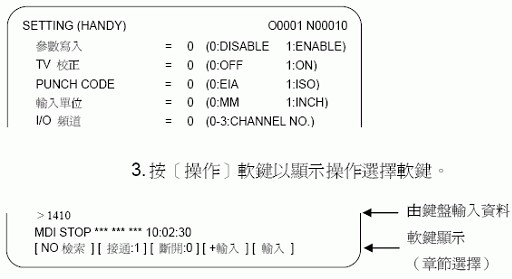
\includegraphics[width=0.9\textwidth]{images/14-1}
	\caption{频道设定} \label{频道设定}
\end{figure}

2关闭CNC系统及机台总电源;

3打开机台电控箱,将安装好的PCMCIA接口的CF卡插入到FANUC 0i主机的【CNMC】插槽,安装时注意方向,不可用力过猛;
如图\ref{插入PCMCIA卡}所示。

\begin{figure}[!hbtp]
	\centering	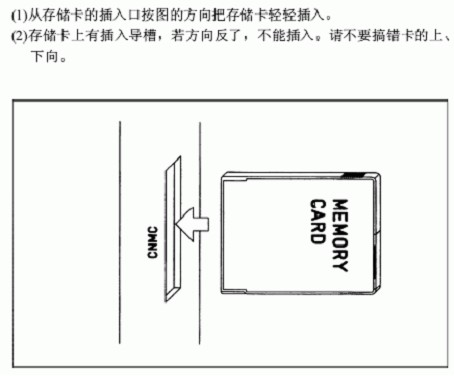
\includegraphics[width=0.9\textwidth]{images/14-2}
	\caption{插入PCMCIA卡} \label{插入PCMCIA卡}
\end{figure}

4进入NC的BOOT界面,方法为:同时按住屏幕下方最右边的两个软建,如图\ref{进入BOOT界面}所示:

\begin{figure}[!hbtp]
\centering	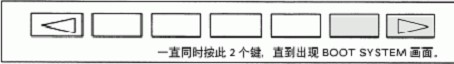
\includegraphics[width=0.9\textwidth]{images/14-3}
\caption{进入BOOT界面1} \label{进入BOOT界面}
\end{figure}

同时开启NC电源,直到出现如图\ref{进入BOOT界面1}的画面:

\begin{figure}[!hbtp]
\centering	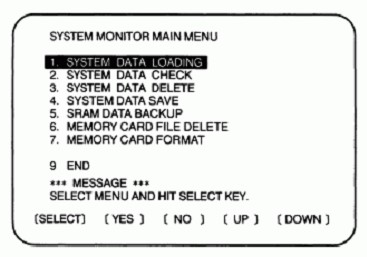
\includegraphics[width=0.9\textwidth]{images/14-4}
\centering	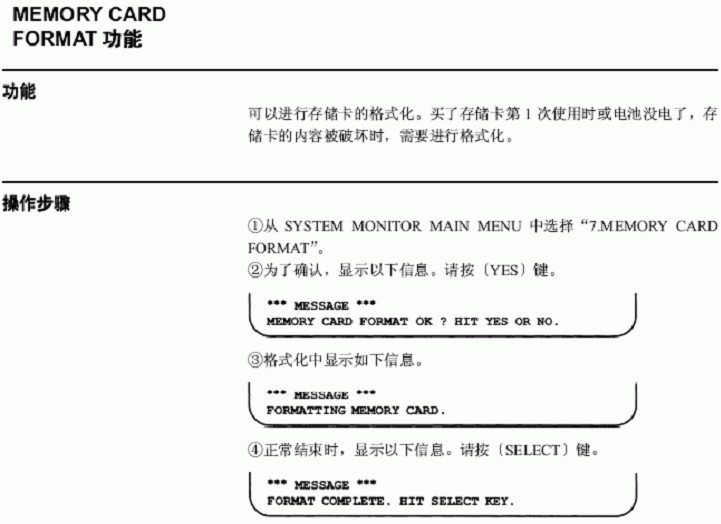
\includegraphics[width=0.9\textwidth]{images/14-5}
\caption{进入BOOT界面2} \label{进入BOOT界面1}
\end{figure}

格式化完成后,退出BOOT界面,重启系统,退出步骤如图\ref{格式化}所示:
\begin{figure}[!hbtp]
	\centering	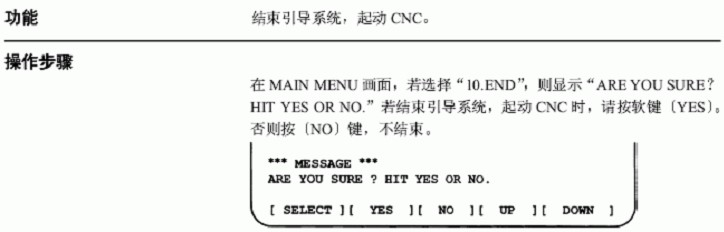
\includegraphics[width=0.9\textwidth]{images/14-6}
	\caption{格式化} \label{格式化}
\end{figure}

如果一切正常,格式过的CF卡,就可以在FANUC0i系统中使用了。如程式的存储,备份,调用等。

(二).PCMCIA卡在FANUC0i系统上的使用

Oi-MB PCMCIA读取程序操作步骤,如图\ref{读取程序操作步骤}所示。
\begin{figure}[!hbtp]
	\centering	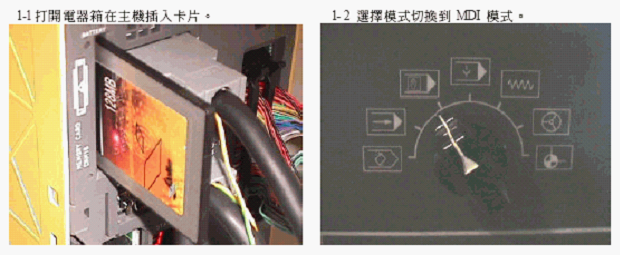
\includegraphics[width=0.8\textwidth]{images/14-7}
%	\caption{格式化} \label{格式化}
\end{figure}

\begin{figure}[!hbtp]
	\centering	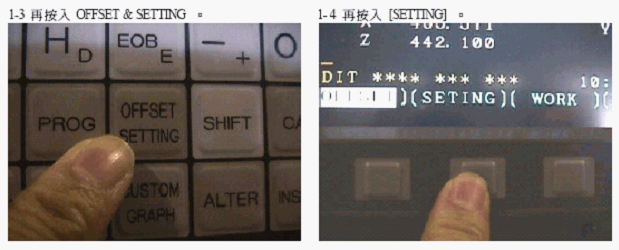
\includegraphics[width=0.8\textwidth]{images/14-8}
	%	\caption{格式化} \label{格式化}
\end{figure}

\begin{figure}[!hbtp]
	\centering	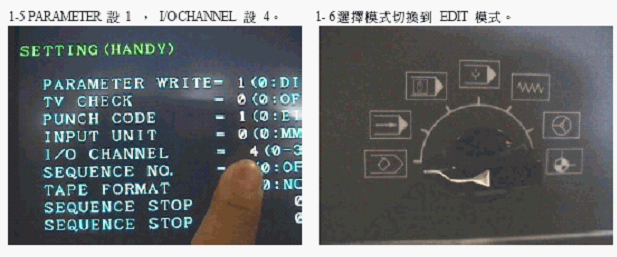
\includegraphics[width=0.8\textwidth]{images/14-9}
	%	\caption{格式化} \label{格式化}
\end{figure}


\begin{figure}[!hbtp]
	\centering	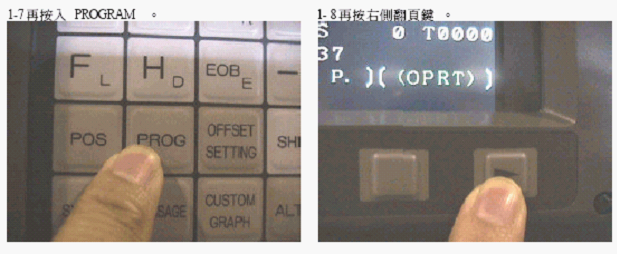
\includegraphics[width=0.8\textwidth]{images/14-10}
	%	\caption{格式化} \label{格式化}
\end{figure}

\begin{figure}[!hbtp]
	\centering	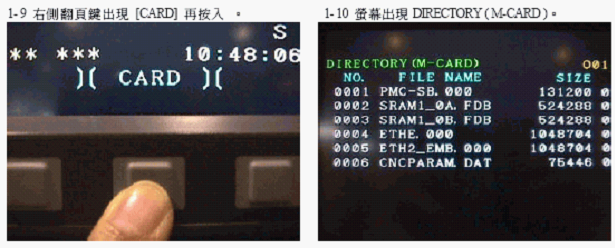
\includegraphics[width=0.8\textwidth]{images/14-11}
	\caption{读取程序操作步骤} \label{读取程序操作步骤}
\end{figure}

将NC记忆体的资料拷贝到(M-CARD)的步骤,如图\ref{NC到M-CARD}所示。

\begin{figure}[!hbtp]
	\centering	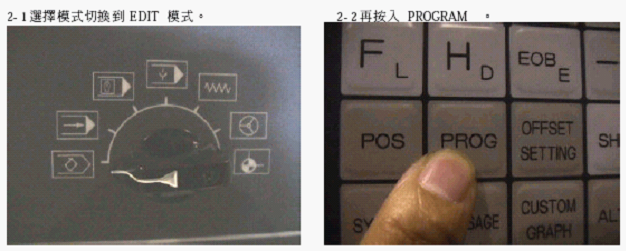
\includegraphics[width=0.8\textwidth]{images/14-12}
	%	\caption{格式化} \label{格式化}
\end{figure}

\begin{figure}[!hbtp]
	\centering	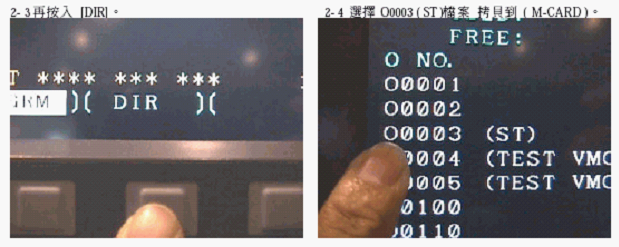
\includegraphics[width=0.8\textwidth]{images/14-13}
	%	\caption{格式化} \label{格式化}
\end{figure}

\begin{figure}[!hbtp]
	\centering	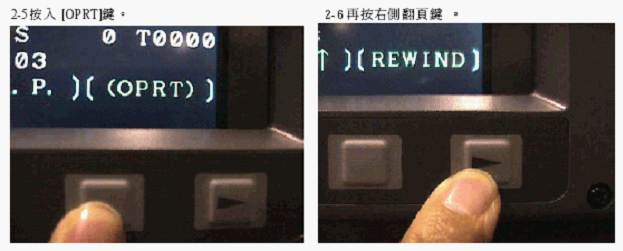
\includegraphics[width=0.8\textwidth]{images/14-14}
	%	\caption{格式化} \label{格式化}
\end{figure}

\begin{figure}[!hbtp]
	\centering	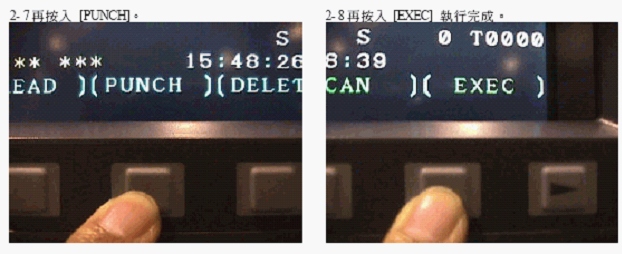
\includegraphics[width=0.8\textwidth]{images/14-15}
	%	\caption{格式化} \label{格式化}
\end{figure}

\begin{figure}[!hbtp]
	\centering	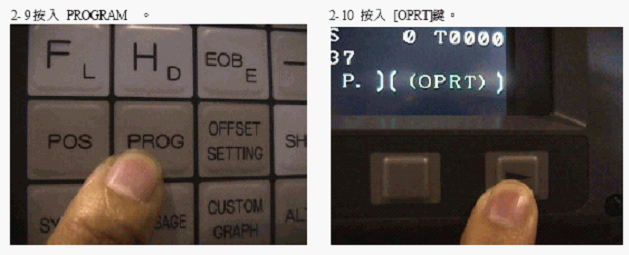
\includegraphics[width=0.8\textwidth]{images/14-16}
	%	\caption{格式化} \label{格式化}
\end{figure}

\begin{figure}[!hbtp]
	\centering	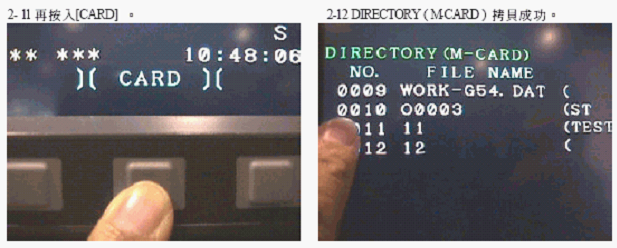
\includegraphics[width=0.8\textwidth]{images/14-17}
	\caption{NC到M-CARD} \label{NC到M-CARD}
\end{figure}

将(M-CARD)资料拷贝到NC记忆体的步骤,如图\ref{M-CARD到NC}所示。

\begin{figure}[!hbtp]
	\centering	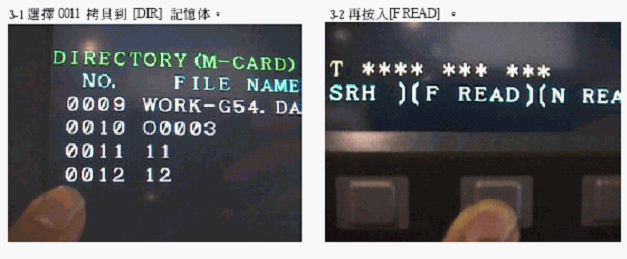
\includegraphics[width=0.8\textwidth]{images/14-18}
%	\caption{NC到M-CARD} \label{NC到M-CARD}
\end{figure}

\begin{figure}[!hbtp]
	\centering	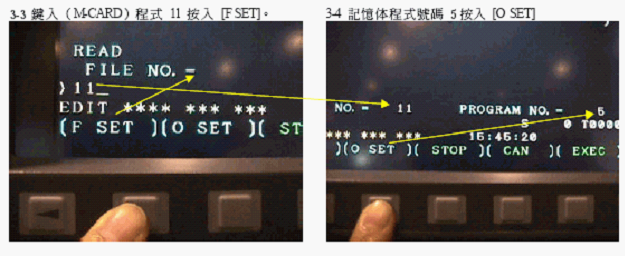
\includegraphics[width=0.8\textwidth]{images/14-19}
	%	\caption{NC到M-CARD} \label{NC到M-CARD}
\end{figure}

\begin{figure}[!hbtp]
	\centering	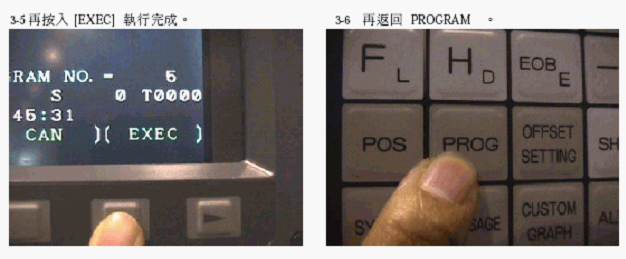
\includegraphics[width=0.8\textwidth]{images/14-20}
	%	\caption{NC到M-CARD} \label{NC到M-CARD}
\end{figure}

\begin{figure}[!hbtp]
	\centering	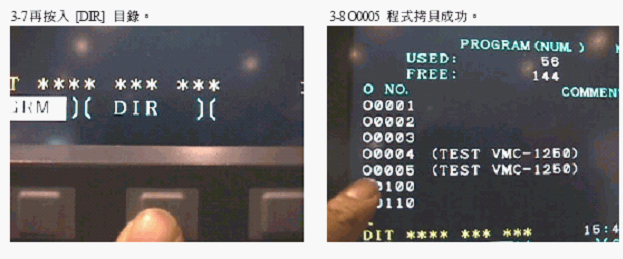
\includegraphics[width=0.8\textwidth]{images/14-21}
	\caption{M-CARD到NC} \label{M-CARD到NC}
\end{figure}

M-CARD程式刪除步骤,如图\ref{程式刪除}所示。

\begin{figure}[!hbtp]
	\centering	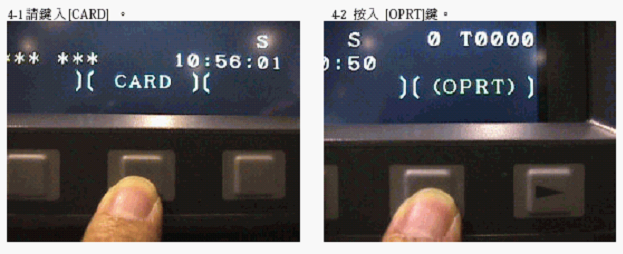
\includegraphics[width=0.8\textwidth]{images/14-22}
%	\caption{M-CARD到NC} \label{M-CARD到NC}
\end{figure}

\begin{figure}[!hbtp]
	\centering	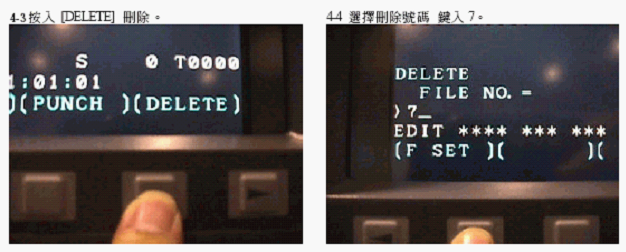
\includegraphics[width=0.8\textwidth]{images/14-23}
%	\caption{M-CARD到NC} \label{M-CARD到NC}
\end{figure}

\begin{figure}[!hbtp]
	\centering	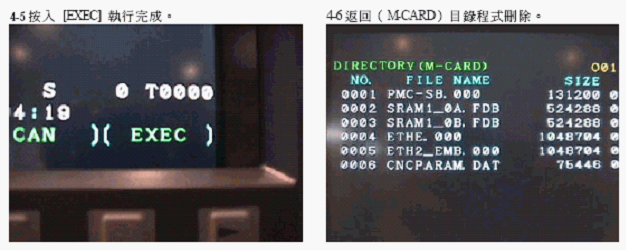
\includegraphics[width=0.8\textwidth]{images/14-24}
	\caption{程式刪除} \label{程式刪除}
\end{figure}
选择(M-CARD)DATA执行,如图\ref{M-CARD执行}所示。

\begin{figure}[!hbtp]
	\centering	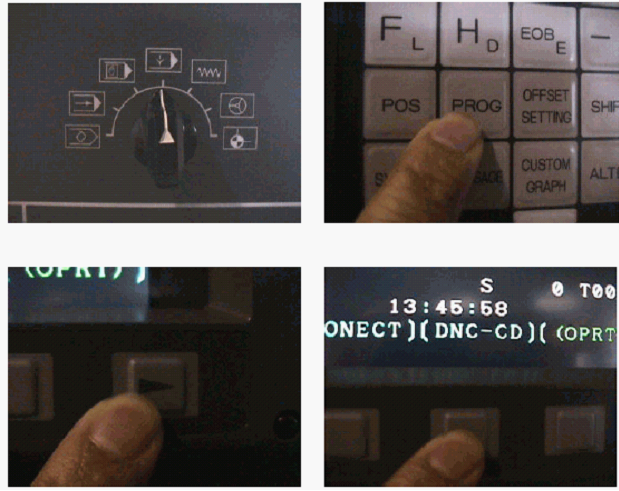
\includegraphics[width=0.8\textwidth]{images/14-25}
%	\caption{程式刪除} \label{程式刪除}
\end{figure}
\begin{figure}[!hbtp]
	\centering	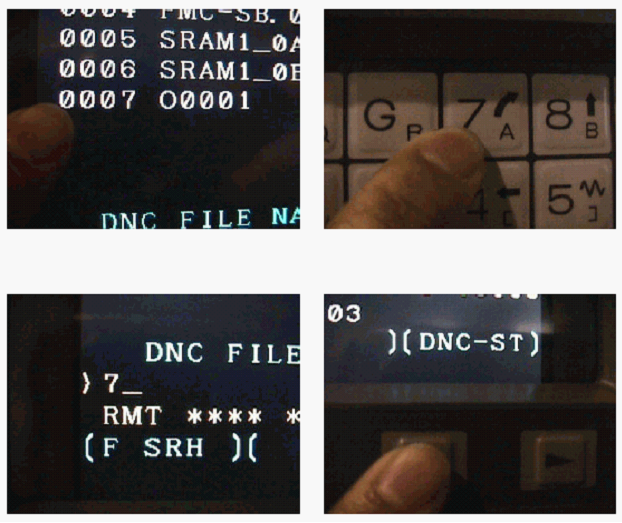
\includegraphics[width=0.8\textwidth]{images/14-26}
%	\caption{程式刪除} \label{程式刪除}
\end{figure}
\begin{figure}[!hbtp]
	\centering	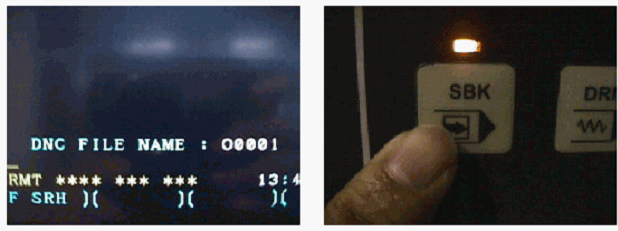
\includegraphics[width=0.8\textwidth]{images/14-27}
	\caption{M-CARD执行} \label{M-CARD执行}
\end{figure}

\newpage
\subsection{课堂小结}
\begin{enumerate}[1、]
	\item 数据线的接法;
	\item 传输过程;
	\item DNC 在线加工。
\end{enumerate}

\vfill
\subsection{布置作业}
\begin{enumerate}[1、]
	\item 写出上面的程序;
	\item 从习题集上选做一个。
\end{enumerate}
\vfill